An interesting property about ladder lotteries is that they can be derived from a 
\emph{permutation} which is a is a unique ordering of objects.
For the purposes on this paper, the objects of a permutation will be integers 
ranging from [$1$ $\dots$ $N$]. \emph{Optimal ladder lotteries} are a special case of ladder 
lotteries in which there is one bar in the ladder for each \emph{inversion} in the permutation.
An \emph{inversion} is a relation between two elements in $\pi$, 
$\pi_{i}$ and $\pi_{j}$, such that if $\pi_{i}>\pi_{j}$ and $i<j$ then $\pi_{i}$ and $\pi_{j}$ 
form an inversion. 
For example, given $\pi=(4,3,5,1,2)$, its iversion set is $Inv(\pi) =\{(4,3),(4,1),(4,2),(3,1),(3,2),(5,1),(5,2)\}$.
Every permutation has a unique, finite set of optimal ladder lotteries associated with it. 
 Thus, the set of optimal ladder lotteries associated with $\pi$, 
 hereby known as \emph{$OptL\{\pi\}$}, is the set containing all ladder lotteries 
 with a number of bars equal to the number if inversions in $\pi$. 
 See Fig. 2.1 for an example of an optimal ladder in $OptL\{(4,3,2,1)\}$.
 For each optimal ladder in $OptL\{\pi\}$, the $N$ 
 elements in $\pi$ are listed at the top of a ladder and each 
 element is given its own line. 
 At the bottom of a ladder is the \emph{sorted permutation}, 
 hereby known as the \emph{identity permutation} \cite{A7}. 
 The  identity permutation of size $N$ is defined as follows - $I:(1, 2, 3, \dots, N)$. 
 Each ladder in $OptL\{\pi\}$ has the minimal number of horizontal bars to sort $\pi$ 
 into the identity permutation. Each bar in a ladder from $OptL\{\pi\}$ uninverts a single 
 inversion in $\pi$ exactly once. For the remainder of this paper, only optimal ladder 
 lotteries will be discussed, with one exception. Therefore when the term ladder lottery is used, assume 
 optimal ladder lottery unless otherwise stated.\par
 
\begin{figure}[!htp]
    \label{fig:ab}
	\begin{minipage}{0.4\textwidth}
		\centering
		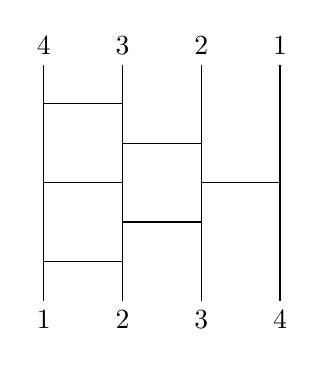
\begin{tikzpicture}
		 	\draw(0, 0) to (0, 3) ++(0, 0) node[above]{4} --(0, 0)node[below]{1};
		 		\draw(0, 2.5) to (1, 2.5);
		 		\draw(0, 1.5) to (1, 1.5);
		 		\draw(0, 0.5) to (1, 0.5);

		 	\draw(1, 0) to (1, 3) ++(0, 0) node[above]{3} --(1, 0)node[below]{2};
		 		\draw(1, 2) to (2, 2);
		 		\draw(1, 1) to (2, 1);
		 	\draw(2, 0) to (2, 3) ++(0, 0) node[above]{2} --(2, 0)node[below]{3};
		 		\draw(2, 1.5) to (3, 1.5);
		 	\draw(3, 0) to (3, 3) ++(0, 0) node[above]{1} --(3, 0) node[below]{4};
		\end{tikzpicture}
				

	\end{minipage}
	\begin{minipage}{.4\textwidth}
		\begin{flushright}
		
		
		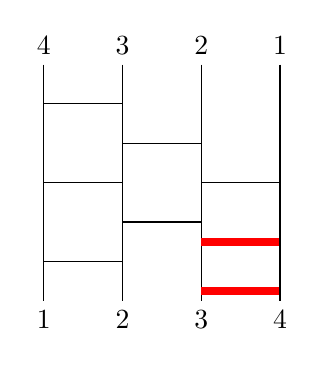
\begin{tikzpicture}
		 	\draw(0, 0) to (0, 3) ++(0, 0) node[above]{4} --(0, 0)node[below]{1};
		 		\draw(0, 2.5) to (1, 2.5);
		 		\draw(0, 1.5) to (1, 1.5);
		 		\draw(0, 0.5) to (1, 0.5);
		 		

		 	\draw(1, 0) to (1, 3) ++(0, 0) node[above]{3} --(1, 0)node[below]{2};
		 		\draw(1, 2) to (2, 2);
		 		\draw(1, 1) to (2, 1);
		 	\draw(2, 0) to (2, 3) ++(0, 0) node[above]{2} --(2, 0)node[below]{3};
		 		\draw(2, 1.5) to (3, 1.5);
		 		\draw[line width=1mm, red](2, 0.75) to (3, 0.75);
		 		\draw[line width=1mm, red](2, 0.125) to (3, 0.125);
		 	\draw(3, 0) to (3, 3) ++(0, 0) node[above]{1} --(3, 0) node[below]{4};
		\end{tikzpicture}
	\end{flushright}
	\end{minipage}
	\caption{Two ladders for the permutation (4, 3, 2, 1). The left ladder is an optimal ladder and the right ladder is not. Therefore the left ladder belongs to $optL\{(4,3,2,1)\}$. The bold  bars in the right ladder are redundant, thus the right ladder is not optimal}
	
\end{figure}


